\documentclass[12pt, a4paper]{report}
\usepackage[top=3cm,left=3cm,right=2cm,bottom=2cm]{geometry}
\linespread{1.3}
\setlength{\parindent}{1.25cm}
\usepackage{indentfirst}
\usepackage[utf8]{inputenc}
\usepackage[brazil]{babel}
\usepackage{amsmath}
\usepackage{amsthm}
\usepackage{amsfonts}
\usepackage{amssymb}
\usepackage{graphicx}
\usepackage{color}
\usepackage{multicol}
\usepackage[normalem]{ulem}
\usepackage{wrapfig}
\usepackage{caption}
\usepackage{fancybox}
\usepackage[pdfstartview=FitH]{hyperref}
\usepackage{subfigure}
\usepackage{algorithm}
\usepackage{algpseudocode}
\usepackage{float}
\usepackage{multirow}
\usepackage{siunitx}
\usepackage{rotating}
\usepackage{booktabs}
\usepackage[table]{xcolor}
\usepackage{array}
\usepackage{colortbl}

\graphicspath{{Figuras/}}

\renewcommand{\theenumii}{\alph{enumii}}
\DeclareMathOperator{\sen}{sen}
\DeclareMathOperator{\tg}{tg}
\DeclareMathOperator{\arctg}{arctg}
\DeclareMathOperator{\cotg}{cotg}
\DeclareMathOperator{\agm}{agm}

\newtheorem{thm}{Teorema}[section]
\newtheorem{dfn}{Definição}[section]
\newtheorem{prob}{Problema}[section]
\newtheorem{cor}{Corolário}[section]
\newtheorem{prop}{Proposição}[section]
\newtheorem{lem}{Lema} [section]

\newcounter{contar}

% Variáveis do projeto
\newcommand{\nomeUniversidade}{Universidade Federal da Bahia}
\newcommand{\nomeInstituto}{Instituto de Computação}
\newcommand{\nomeCurso}{Interação Humano-Computador}
\newcommand{\nomeProfessor}{Prof. Igor Sobral}
\newcommand{\nomeGrupo}{\sc{\large{Antoniel Magalhães (antoniels@ufba.br)}} \\
\sc{\large{André Costa (andre.lino@ufba.br)}} \\
\sc{\large{João Leahy (joao.leahy.ufba.br)}} \\
\sc{\large{Luis Felipe (luis.sena@ufba.br)}} \\
\sc{\large{Koichi Filho (koichifilho@ufba.br)}}
}
\newcommand{\titulo}{\sc{\Large{Projeto Prático Final: Sistema de Gestão de Monitorias (SIGA-M)}}}

\begin{document}

% Capa
\pagestyle{empty}
\begin{center}

\includegraphics[height=2.5cm]{UFBA.jpg}
\hspace{2cm}
\end{center}

\begin{center}
\sc{\large{\nomeUniversidade}} \\
\sc{\large{\nomeInstituto}} \\
\sc{\small{\nomeCurso}} \\

\vspace{4cm}

\titulo

\vspace{4.5cm}

\nomeGrupo

\vspace{5.5cm}

\textbf{Salvador - Bahia} \\
13 de julho de 2025
\end{center}

% Folha de rosto
\newpage
\begin{center}
\titulo

\vspace{4cm}

\nomeGrupo
\end{center}

\vspace{4cm}

\begin{flushright}
\begin{minipage}{8.6cm}
Projeto prático final apresentado ao professor \nomeProfessor\ 
como método avaliativo da disciplina \nomeCurso.
\end{minipage}
\end{flushright}
 
\vspace{8cm}

\begin{center}
\textbf{Salvador - Bahia} \\
13 de julho de 2025
\end{center}

% Índice
\newpage
\tableofcontents
\thispagestyle{empty}
\newpage
\setcounter{page}{1}
\pagestyle{plain}

\chapter{Etapa 1: Análise (Situação atual)}
\label{ch:analise}

\section{Tema e Objetivo Geral do Projeto}

O presente projeto visa realizar o design de IHC para o Sistema de Gestão de Monitorias (SIGA-M), uma plataforma computacional interativa destinada a otimizar os processos administrativos do programa de monitoria do Instituto de Computação (IC) da UFBA.

O objetivo geral é projetar uma solução que automatize e centralize as tarefas envolvidas no ciclo de vida da monitoria — desde a submissão dos projetos pelos professores até o cadastro final dos monitores selecionados. O foco do trabalho está no design da interface e da interação, buscando reduzir a carga de trabalho manual, minimizar erros e melhorar a comunicação entre os envolvidos (comissão de monitoria, professores e alunos).

\section{Identificação das Necessidades e Requisitos de IHC}

\subsection{Levantamento das Necessidades dos Estudantes}

O levantamento de necessidades foi realizado a partir de uma entrevista com um membro da comissão de monitoria, que atua como principal stakeholder do processo. As dores e necessidades identificadas são:

\begin{itemize}
    \item \textbf{Processo Manual e Repetitivo}: A criação de projetos de monitoria a cada semestre é manual. Professores precisam preencher documentos com informações que raramente mudam, copiando dados de editais anteriores.
    
    \item \textbf{Dificuldade de Gestão e Acompanhamento}: A comissão de monitoria enfrenta dificuldades para rastrear quais professores já enviaram seus projetos assinados, dependendo de planilhas e comunicação via e-mail.
    
    \item \textbf{Comunicação Fragmentada}: O envio de lembretes e a cobrança de pendências são feitos manualmente, consumindo tempo e energia da comissão.
    
    \item \textbf{Consolidação de Dados}: A geração da planilha final com todos os projetos para a Pró-Reitoria de Graduação (PROGRAD) é um trabalho manual de consolidação de múltiplos arquivos e links.
    
    \item \textbf{Fluxo de Trabalho Descentralizado}: O processo atual envolve múltiplos arquivos (DOCX, PDF), planilhas, e-mails e pastas em drives compartilhados, aumentando o risco de erros e perda de informação.
\end{itemize}

\subsection{Definição dos Requisitos de IHC}

Com base nas necessidades, foram definidos os seguintes requisitos para o SIGA-M:

\subsubsection{Requisitos Funcionais}

\begin{itemize}
    \item O sistema deve possuir três perfis de usuário: Administrador (comissão de monitoria), Professor e Aluno.
    
    \item Deve ser possível para o Administrador iniciar um novo ciclo de monitoria, importando a planilha de planejamento do semestre.
    
    \item O sistema deve gerar automaticamente os documentos de projeto de monitoria para cada disciplina, pré-preenchendo dados do professor, da disciplina e de um histórico de projetos.
    
    \item O Professor deve poder revisar, editar (se necessário), baixar o projeto para assinatura e fazer o upload do documento assinado.
    
    \item O Administrador deve ter um painel para visualizar o status de submissão de todos os projetos em tempo real.
    
    \item O Administrador deve poder enviar e-mails de lembrete (individualmente ou em massa) para professores com pendências.
    
    \item O sistema deve gerar a planilha final de projetos (para a PROGRAD) no formato exigido, com links para os documentos assinados.
\end{itemize}

\subsubsection{Requisitos Não-Funcionais}

\begin{itemize}
    \item \textbf{Usabilidade}: A interface deve ser clara e direta, permitindo que professores com diferentes níveis de familiaridade com tecnologia completem suas tarefas de forma rápida e eficiente.
    
    \item \textbf{Confiabilidade}: O sistema deve ser estável e garantir a integridade dos dados e documentos submetidos.
    
    \item \textbf{Segurança}: Dados sensíveis de professores e alunos (CPF, dados bancários, etc.) devem ser armazenados e transmitidos de forma segura.
\end{itemize}

\subsection{Matriz de Requisitos por Perfil de Usuário}

A tabela a seguir apresenta uma visão consolidada dos requisitos funcionais organizados por perfil de usuário, facilitando a compreensão das responsabilidades e permissões de cada tipo de usuário no sistema.

\begin{table}[H]
\centering
\caption{Comparação de Requisitos Funcionais por Perfil de Usuário}
\label{tab:requisitos-perfil}
\renewcommand{\arraystretch}{1.2}
\begin{tabular}{|p{4cm}|c|c|c|c|}
\hline
\textbf{Funcionalidade} & \textbf{Professor} & \textbf{Administrador} & \textbf{Estudante} & \textbf{Prioridade} \\
\hline
Login/Autenticação & \cellcolor{green!30}Sim & \cellcolor{green!30}Sim & \cellcolor{green!30}Sim & Alta \\
\hline
Visualizar projetos & \cellcolor{green!30}Sim & \cellcolor{green!30}Sim & \cellcolor{green!30}Sim & Alta \\
\hline
Criar projetos & \cellcolor{red!30}Não & \cellcolor{green!30}Sim & \cellcolor{red!30}Não & Alta \\
\hline
Submeter projetos & \cellcolor{green!30}Sim & \cellcolor{red!30}Não & \cellcolor{red!30}Não & Alta \\
\hline
Enviar lembretes & \cellcolor{red!30}Não & \cellcolor{green!30}Sim & \cellcolor{red!30}Não & Média \\
\hline
Candidatar-se & \cellcolor{red!30}Não & \cellcolor{red!30}Não & \cellcolor{green!30}Sim & Alta \\
\hline
Gerar relatórios & \cellcolor{red!30}Não & \cellcolor{green!30}Sim & \cellcolor{red!30}Não & Média \\
\hline
\end{tabular}
\end{table}

\section{Organização do Espaço do Problema}

\subsection{Personas}

Foram criadas duas personas para representar os perfis de usuários centrais no primeiro módulo do sistema:

\subsubsection{Persona 1: Prof. Roberto (Coordenador da Monitoria)}

\begin{center}
\fcolorbox{blue!50}{blue!10}{
\begin{minipage}{0.8\textwidth}
\vspace{0.5cm}
\begin{center}
{\Large \textbf{Prof. Roberto (45 anos)}}
\end{center}
\vspace{0.3cm}

\noindent \textbf{Objetivo:} Automatizar gestão de monitoria

\noindent \textbf{Frustração:} Processo manual repetitivo

\noindent \textbf{Nível Tech:} Alto

\noindent \textbf{Disponibilidade:} Limitada

\noindent \textbf{Motivação:} Eficiência e mais bolsas para alunos

\vspace{0.3cm}
\end{minipage}
}
\end{center}

\vspace{0.5cm}

\begin{itemize}
    \item \textbf{Ocupação}: Professor do Instituto de Computação e membro da comissão de monitoria.
    \item \textbf{Perfil}: Roberto é proativo e tecnologicamente competente. Ele dedica um tempo considerável à gestão do programa de monitoria e busca ativamente formas de otimizar o processo, pois sabe que um maior número de projetos submetidos resulta em mais bolsas para os alunos do instituto.
    \item \textbf{Citação}: "Todo semestre é a mesma correria. Tenho que ficar conferindo planilhas, mandando e-mails de cobrança e torcendo para não ter esquecido de ninguém. É um trabalho manual que poderia ser facilmente automatizado."
\end{itemize}

\subsubsection{Persona 2: Profa. Ana (Professora Responsável por Disciplina)}

\begin{center}
\fcolorbox{purple!50}{purple!10}{
\begin{minipage}{0.8\textwidth}
\vspace{0.5cm}
\begin{center}
{\Large \textbf{Profa. Ana (38 anos)}}
\end{center}
\vspace{0.3cm}

\noindent \textbf{Objetivo:} Submissão rápida e simples

\noindent \textbf{Frustração:} Documentos perdidos/retrabalho

\noindent \textbf{Nível Tech:} Médio

\noindent \textbf{Disponibilidade:} Muito limitada

\noindent \textbf{Motivação:} Cumprir obrigação eficientemente

\vspace{0.3cm}
\end{minipage}
}
\end{center}

\vspace{0.5cm}

\begin{itemize}
    \item \textbf{Ocupação}: Professora do Instituto de Computação.
    \item \textbf{Perfil}: Ana é uma professora dedicada, com uma agenda cheia de aulas, reuniões e orientações de pesquisa. Ela valoriza o programa de monitoria, mas vê o processo burocrático de submissão do projeto como mais uma tarefa administrativa em sua longa lista de afazeres.
    \item \textbf{Citação}: "Eu nunca lembro onde salvei o arquivo do semestre passado. Acabo tendo que preencher tudo de novo, mesmo sabendo que a descrição da monitoria de Algoritmos não muda quase nada de um ano para o outro."
\end{itemize}

\subsection{Cenários}

A seguir, apresentamos cenários de uso detalhados para cada persona, com fluxogramas que ilustram visualmente os passos e decisões envolvidos no processo.

\subsubsection{Cenário 1: Prof. Roberto iniciando o ciclo de monitoria}

\begin{figure}[H]
\centering
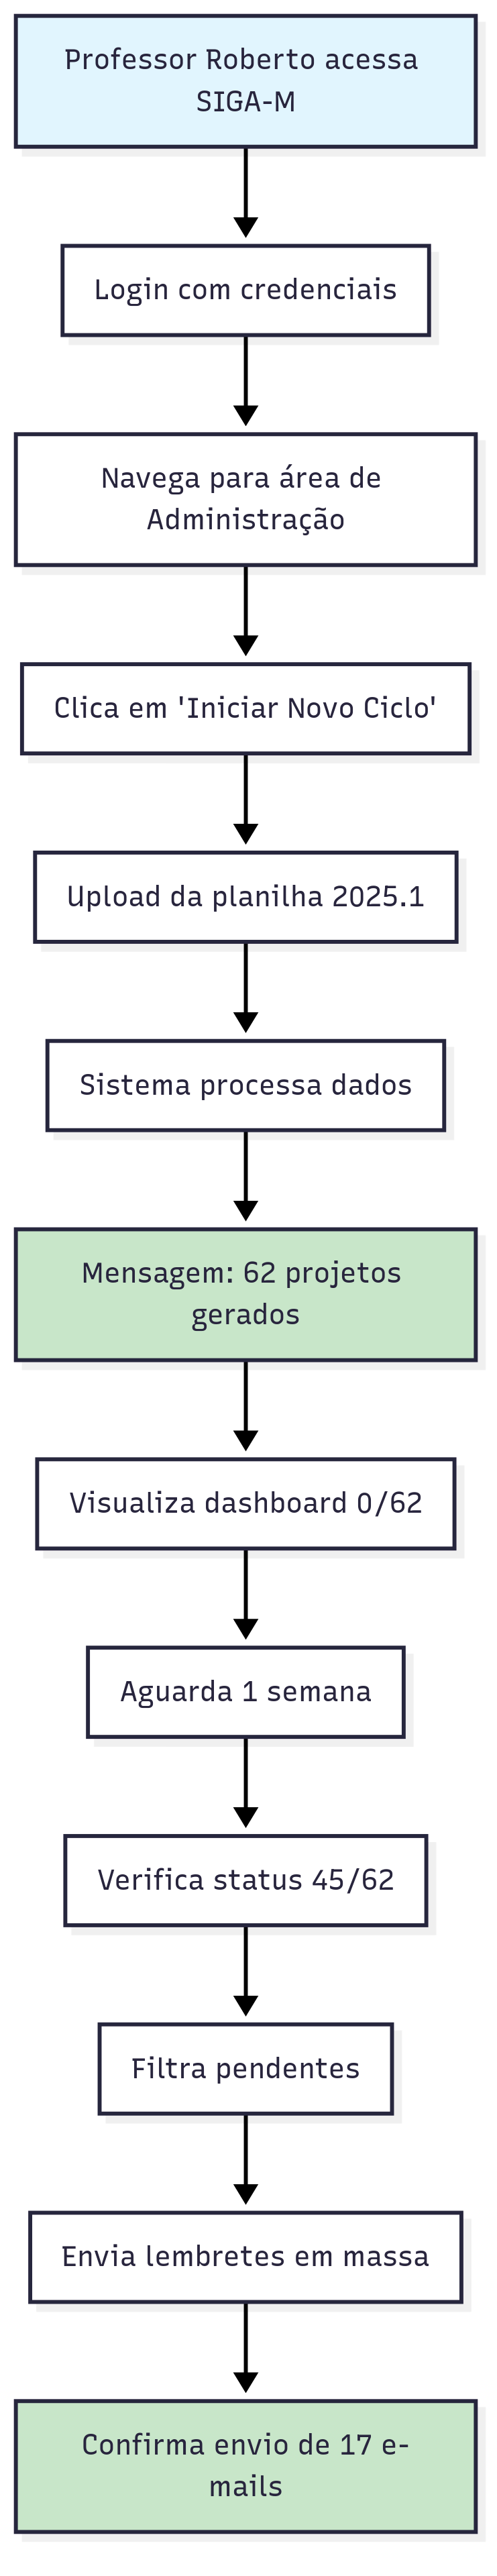
\includegraphics[width=0.2\textwidth]{roberto.png}
\caption{Fluxo de interação do Prof. Roberto iniciando um novo ciclo de monitoria}
\label{fig:cenario-roberto}
\end{figure}

\textbf{Descrição narrativa:}
Roberto acessa o SIGA-M e navega para a área de Administração. Ele clica em "Iniciar Novo Ciclo de Monitoria". O sistema solicita a planilha de planejamento do semestre 2025.1. Ele faz o upload do arquivo. Em poucos segundos, o sistema exibe uma mensagem: "Ciclo 2025.1 iniciado com sucesso. 62 projetos de monitoria gerados e notificações enviadas aos professores responsáveis."

Em seu painel, Roberto vê o status "Projetos Submetidos: 0/62". Uma semana depois, ele acessa novamente o painel, que agora marca "45/62". Ele filtra a lista para exibir apenas os professores com status "Pendente" e clica no botão "Enviar Lembrete para Todos os Pendentes". O sistema confirma o envio de 17 e-mails de lembrete.

\subsubsection{Cenário 2: Profa. Ana submetendo seu projeto}

\begin{figure}[H]
\centering
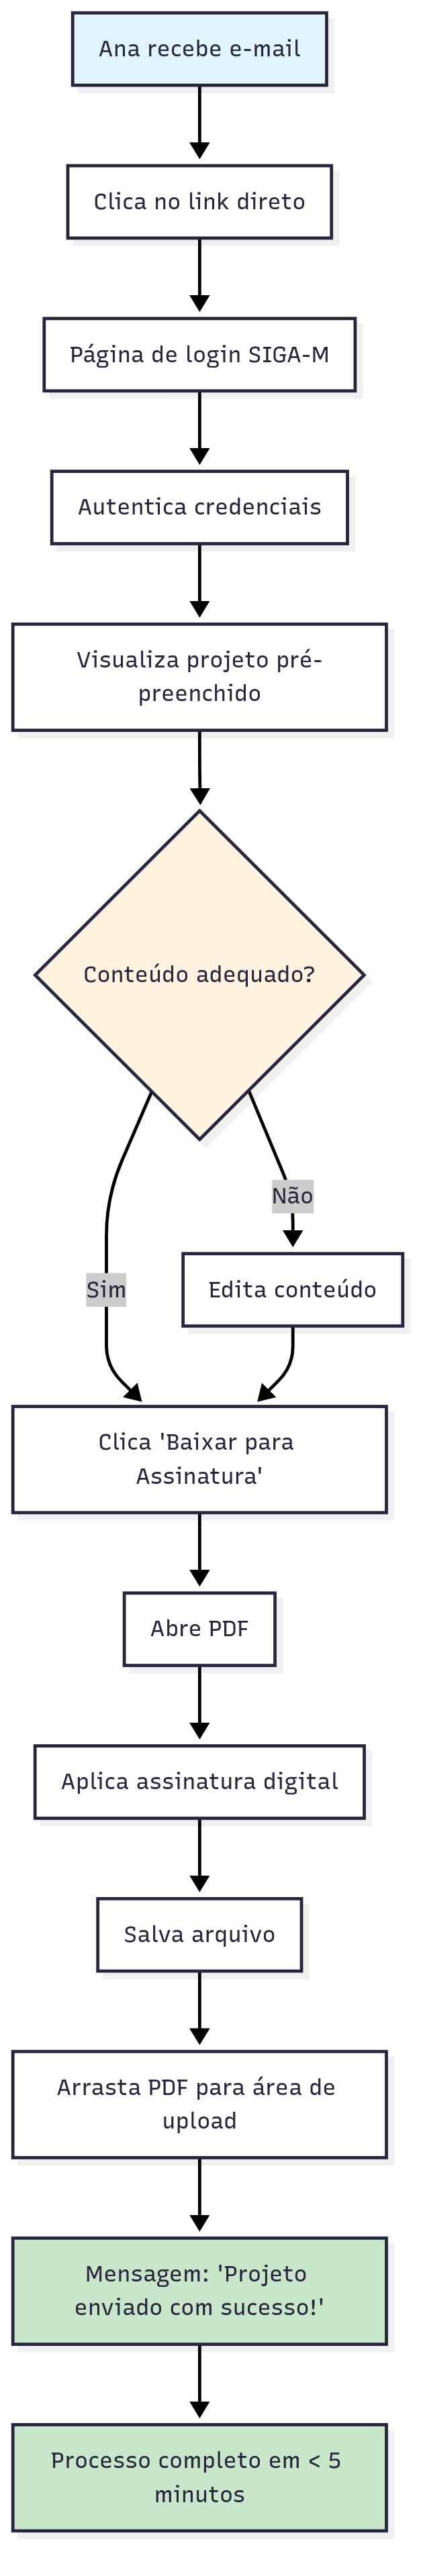
\includegraphics[width=0.2\textwidth]{ana.png}
\caption{Fluxo de submissão de projeto pela Profa. Ana}
\label{fig:cenario-ana}
\end{figure}

\textbf{Descrição narrativa:}
Ana recebe um e-mail com o assunto "SIGA-M: Seu projeto de monitoria para a disciplina de Algoritmos e Estrutura de Dados I está pronto". O e-mail contém um link direto. Ao clicar, ela é levada à página de login do SIGA-M. Após se autenticar, ela vê o documento de seu projeto já preenchido. Ela lê rapidamente e concorda com o conteúdo, que é o mesmo do ano anterior. Ela clica em "Baixar para Assinatura", abre o PDF, aplica sua assinatura digital e salva o arquivo. Em seguida, na mesma página, ela arrasta e solta o PDF assinado na área indicada. Uma mensagem de sucesso aparece: "Projeto enviado com sucesso!". O processo inteiro levou menos de cinco minutos.

\subsection{Análise Hierárquica de Tarefas (HTA)}

A Análise Hierárquica de Tarefas apresenta a decomposição estruturada do objetivo principal do professor no sistema SIGA-M. O diagrama a seguir ilustra visualmente a hierarquia de tarefas e subtarefas envolvidas no processo de submissão de projetos de monitoria.

\begin{figure}[H]
\centering
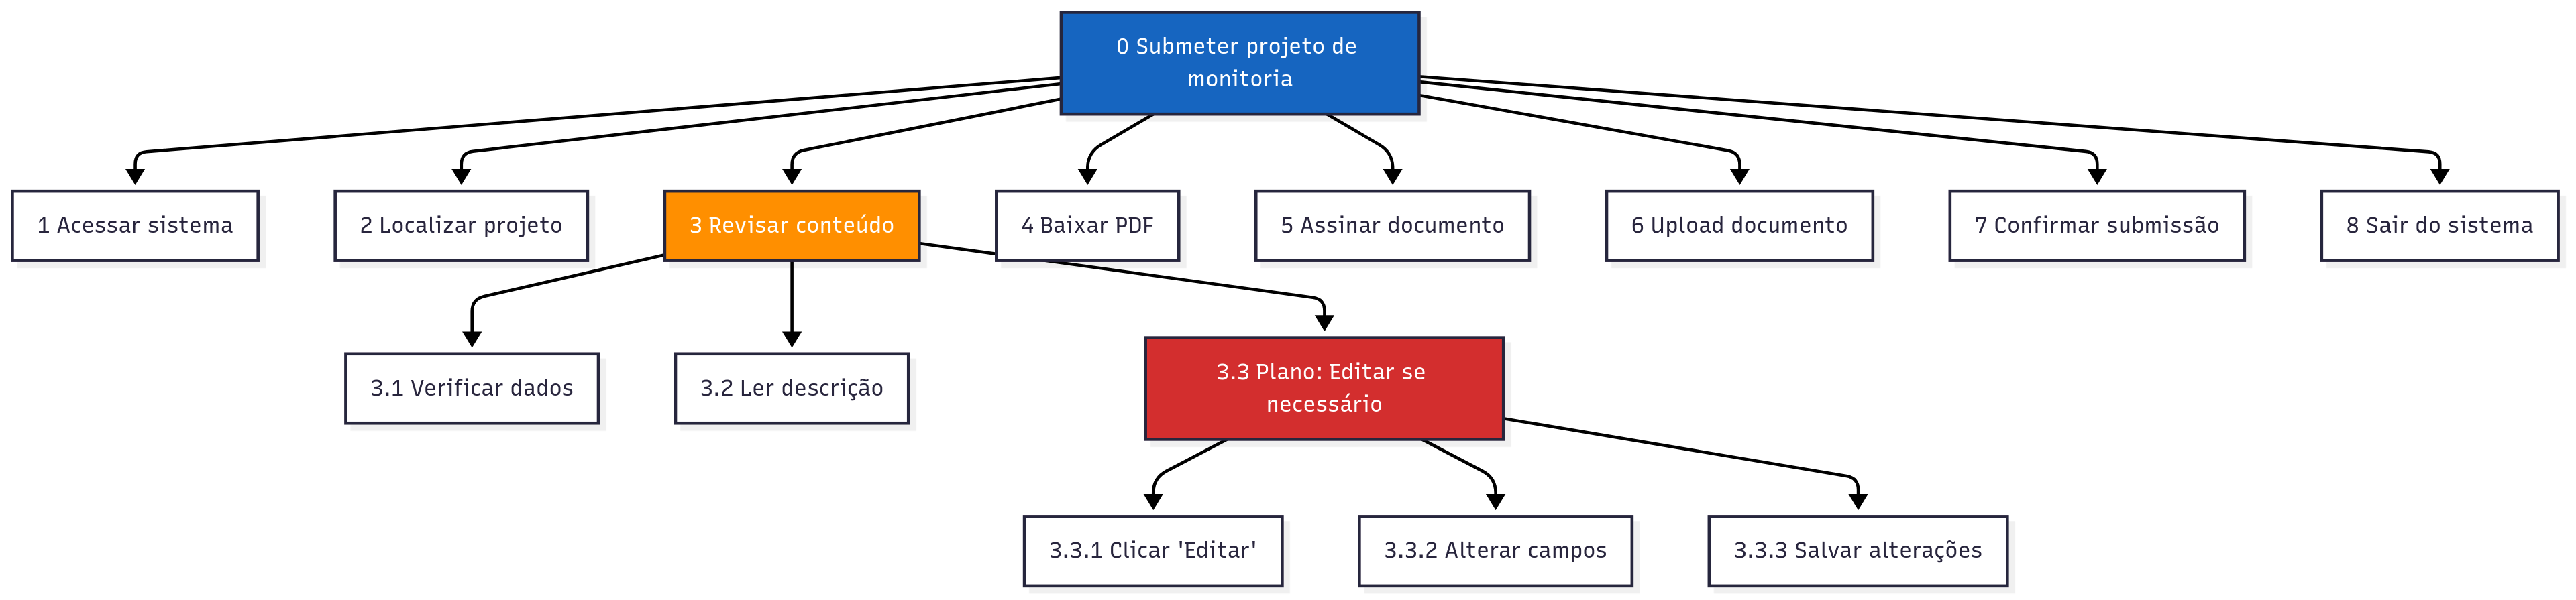
\includegraphics[width=0.95\textwidth]{hta.png}
\caption{Análise Hierárquica de Tarefas - Submeter projeto de monitoria}
\label{fig:hta-diagram}
\end{figure}

\textbf{Objetivo principal}: Submeter o projeto de monitoria

\textbf{Planos de ação}:
\begin{itemize}
    \item \textbf{Plano 0}: Executar tarefas 1-8 em sequência
    \item \textbf{Plano 3}: Se dados estiverem incorretos ou incompletos na tarefa 3.1 ou 3.2, executar 3.3
    \item \textbf{Plano 3.3}: Executar 3.3.1, 3.3.2 e 3.3.3 em sequência
\end{itemize}

\textbf{Condições de ativação}:
\begin{itemize}
    \item A tarefa 3.3 (edição) só é executada se o conteúdo não estiver adequado
    \item A confirmação (tarefa 7) só ocorre após upload bem-sucedido
    \item O usuário pode sair do sistema (tarefa 8) a qualquer momento após a confirmação
\end{itemize}

\chapter{Etapa 2: Síntese (Intervenção)}
\label{ch:sintese}

Esta etapa apresenta a proposta de intervenção sob a forma de um protótipo interativo do sistema SIGA-M, focando no fluxo essencial entre coordenador e professor para o ciclo de criação e aprovação de projetos de monitoria.

\section{Modelo de Interação}

O modelo de interação apresenta o fluxo simplificado de navegação entre as telas principais do sistema, concentrando-se no processo fundamental de criação, submissão e aprovação de projetos de monitoria. O desenvolvimento partiu de um protótipo de baixa fidelidade (Figura \ref{fig:excalidraw}) que estabeleceu as bases para o design final.

\begin{figure}[H]
\centering
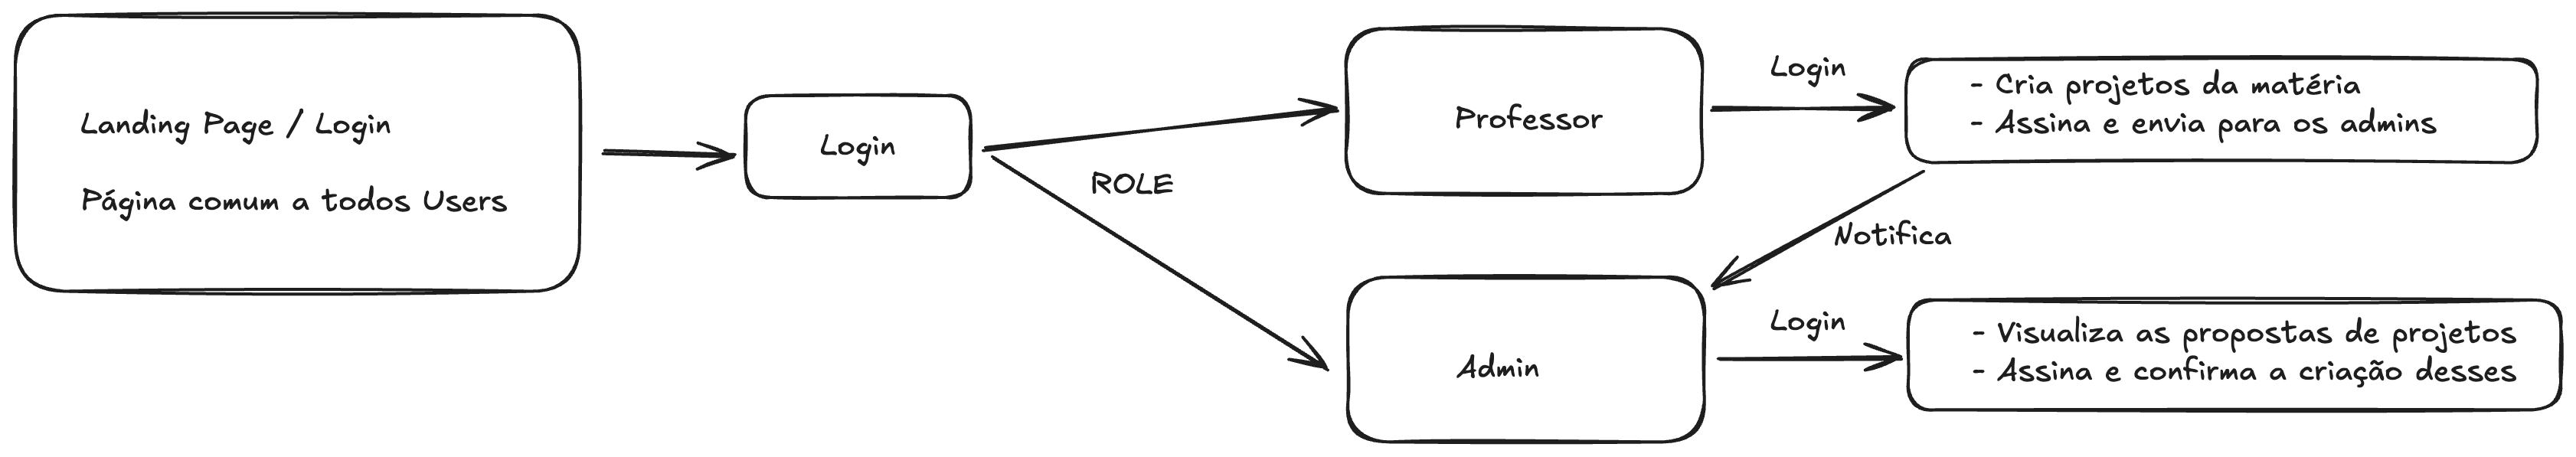
\includegraphics[width=0.8\textwidth]{figma/excalidraw-design.png}
\caption{Protótipo de baixa fidelidade - Base inicial do design}
\label{fig:excalidraw}
\end{figure}

O fluxo principal simplificado segue duas jornadas essenciais:
\begin{itemize}
    \item \textbf{Jornada do Professor}: Login → Criar/Editar Projeto → Enviar Projeto
    \item \textbf{Jornada do Administrador}: Login → Visualizar Projetos → Aprovar/Assinar → Iniciar Processo de Bolsa
\end{itemize}

\subsection{Fluxo de Interação Principal}

O modelo de interação foi otimizado para os dois perfis principais:

\subsubsection{Fluxo do Professor}
\begin{enumerate}
    \item \textbf{Login}: Autenticação via credenciais institucionais
    \item \textbf{Dashboard}: Visualização de projetos existentes ou opção de criar novo
    \item \textbf{Criação de Projeto}: Formulário com dados pré-preenchidos quando disponíveis
    \item \textbf{Revisão}: Verificação das informações do projeto
    \item \textbf{Envio}: Submissão do projeto para aprovação do coordenador
    \item \textbf{Confirmação}: Feedback visual de sucesso no envio
\end{enumerate}

\subsubsection{Fluxo do Administrador (Coordenador)}
\begin{enumerate}
    \item \textbf{Login}: Acesso com perfil administrativo
    \item \textbf{Dashboard}: Visão geral de todos os projetos submetidos
    \item \textbf{Análise}: Revisão detalhada de cada projeto
    \item \textbf{Aprovação}: Assinatura digital e aprovação do projeto
    \item \textbf{Inicialização}: Ativação do processo de bolsa de monitoria
    \item \textbf{Notificação}: Sistema notifica automaticamente os envolvidos
\end{enumerate}

\subsection{Tratamento de Erros e Recuperação}

O sistema implementa mecanismos essenciais de tratamento de erros:

\begin{itemize}
    \item \textbf{Validação de Login}: Feedback claro para credenciais inválidas
    \item \textbf{Salvamento Automático}: Prevenção de perda de dados durante criação de projetos
    \item \textbf{Confirmações}: Diálogos de confirmação antes de ações críticas
    \item \textbf{Navegação Segura}: Sempre com opção de voltar sem perder progresso
\end{itemize}

\section{Link de Acesso ao Protótipo}

O protótipo interativo está disponível na plataforma Figma através do seguinte link:

\url{https://www.figma.com/design/meTbBaQdqBHlvtzBEb9ehF/Sistema-de-Monitoria-IC?node-id=1-2&p=f}

O protótipo permite a simulação completa do fluxo simplificado professor-coordenador, possibilitando a navegação interativa pelas funcionalidades essenciais do sistema.

\section{Vídeo-Demo do Sistema}

O vídeo demonstrativo do sistema SIGA-M está disponível através do seguinte link:

\textbf{TODO: [INSERIR\_LINK\_DO\_VIDEO\_AQUI]}

O vídeo apresenta a explanação oral do projeto e uma demonstração completa do protótipo, mostrando os principais fluxos de interação e funcionalidades do sistema.

\section{Telas e Decisões de Projeto}

As capturas de tela do protótipo e as justificativas das decisões de design são apresentadas a seguir, focando no fluxo principal:

\subsection{Tela de Login}

\begin{figure}[H]
\centering
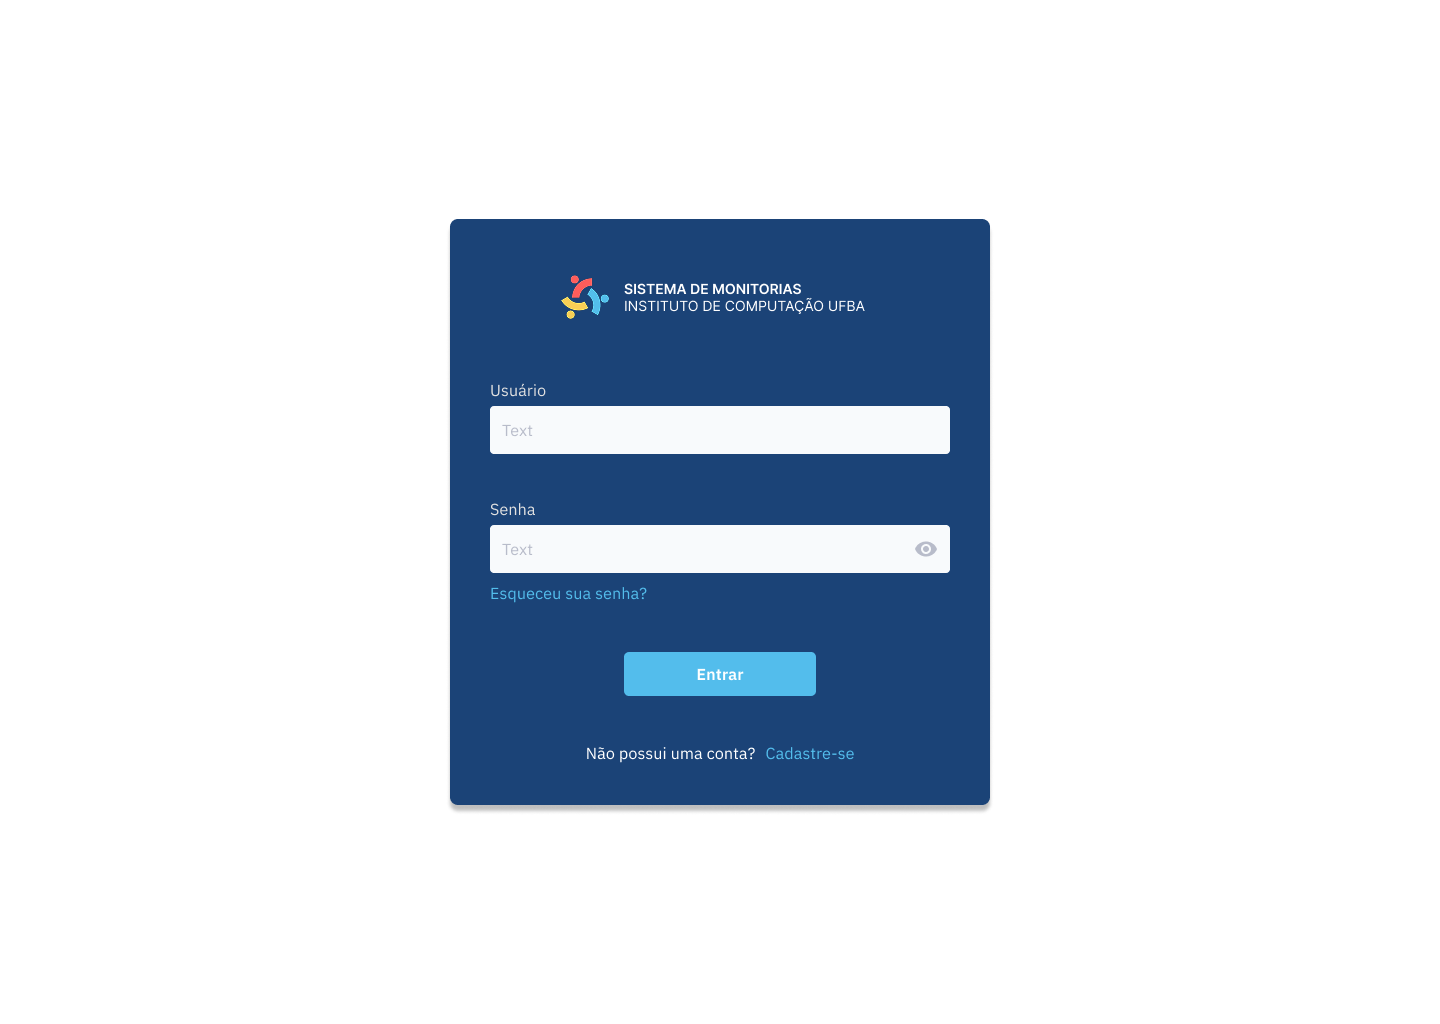
\includegraphics[width=0.8\textwidth]{figma/Login.png}
\caption{Tela de Login do Sistema SIGA-M}
\label{fig:login}
\end{figure}

\textbf{Decisões de Design}:
\begin{itemize}
    \item \textbf{Identidade Visual}: Utilização das cores institucionais da UFBA (azul) para criar familiaridade
    \item \textbf{Simplicidade}: Layout limpo com foco nos campos essenciais
    \item \textbf{Diferenciação de Perfis}: Login único com identificação automática do tipo de usuário
    \item \textbf{Segurança Visual}: Campo de senha com opção de visualização
\end{itemize}

\subsection{Formulário de Criação de Projeto}

\begin{figure}[H]
\centering
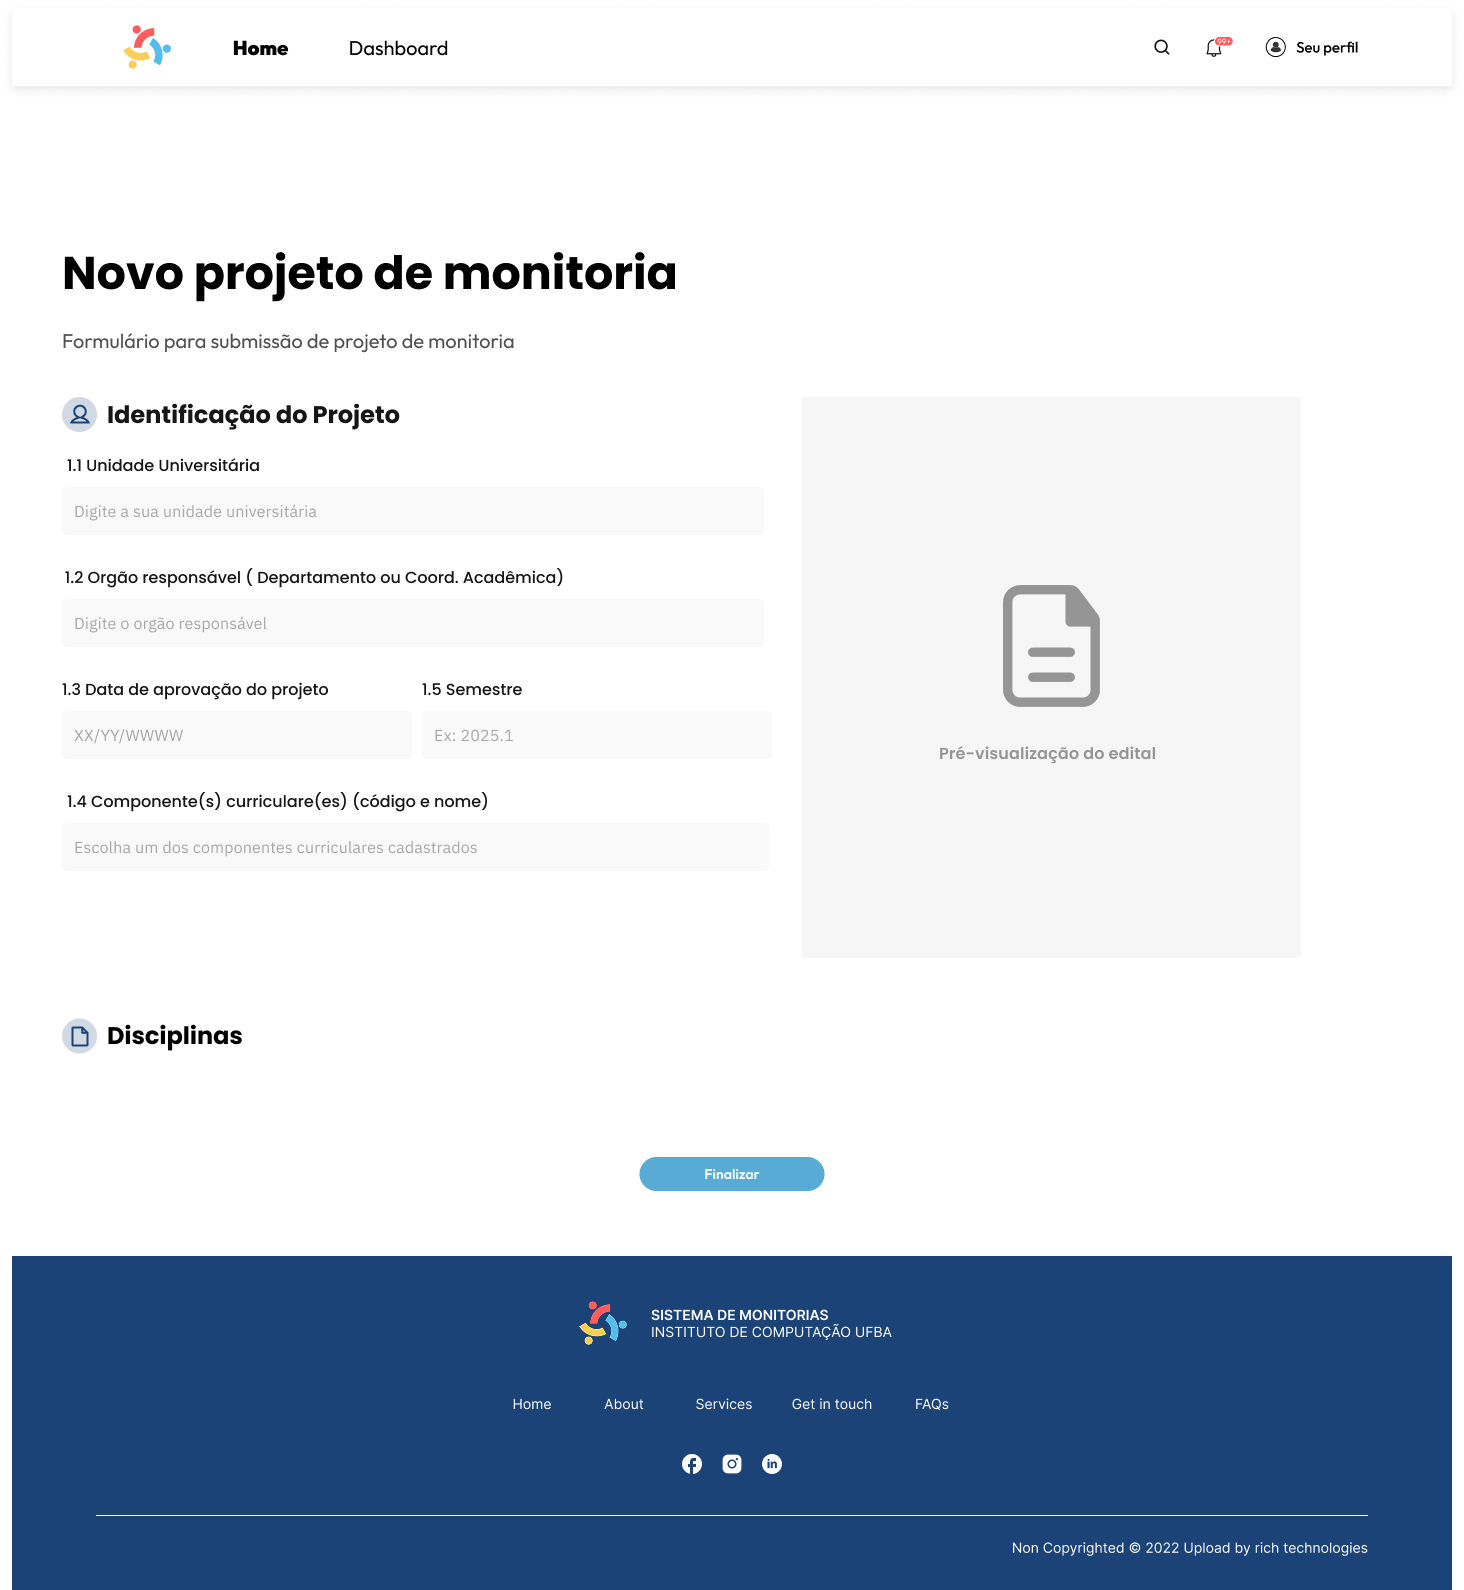
\includegraphics[width=0.9\textwidth]{figma/projeto-monitoria.png}
\caption{Interface de Criação de Projeto de Monitoria}
\label{fig:projeto-monitoria}
\end{figure}

\textbf{Decisões de Design}:
\begin{itemize}
    \item \textbf{Formulário Estruturado}: Campos organizados logicamente seguindo o fluxo do documento oficial
    \item \textbf{Pré-preenchimento Inteligente}: Dados do professor e histórico carregados automaticamente
    \item \textbf{Validação em Tempo Real}: Indicadores visuais de campos obrigatórios e validados
    \item \textbf{Ações Claras}: Botões de "Salvar Rascunho" e "Enviar para Aprovação" bem posicionados
    \item \textbf{Navegação Contextual}: Breadcrumb indicando posição no processo
\end{itemize}

\subsection{Dashboard do Coordenador}

\begin{figure}[H]
\centering
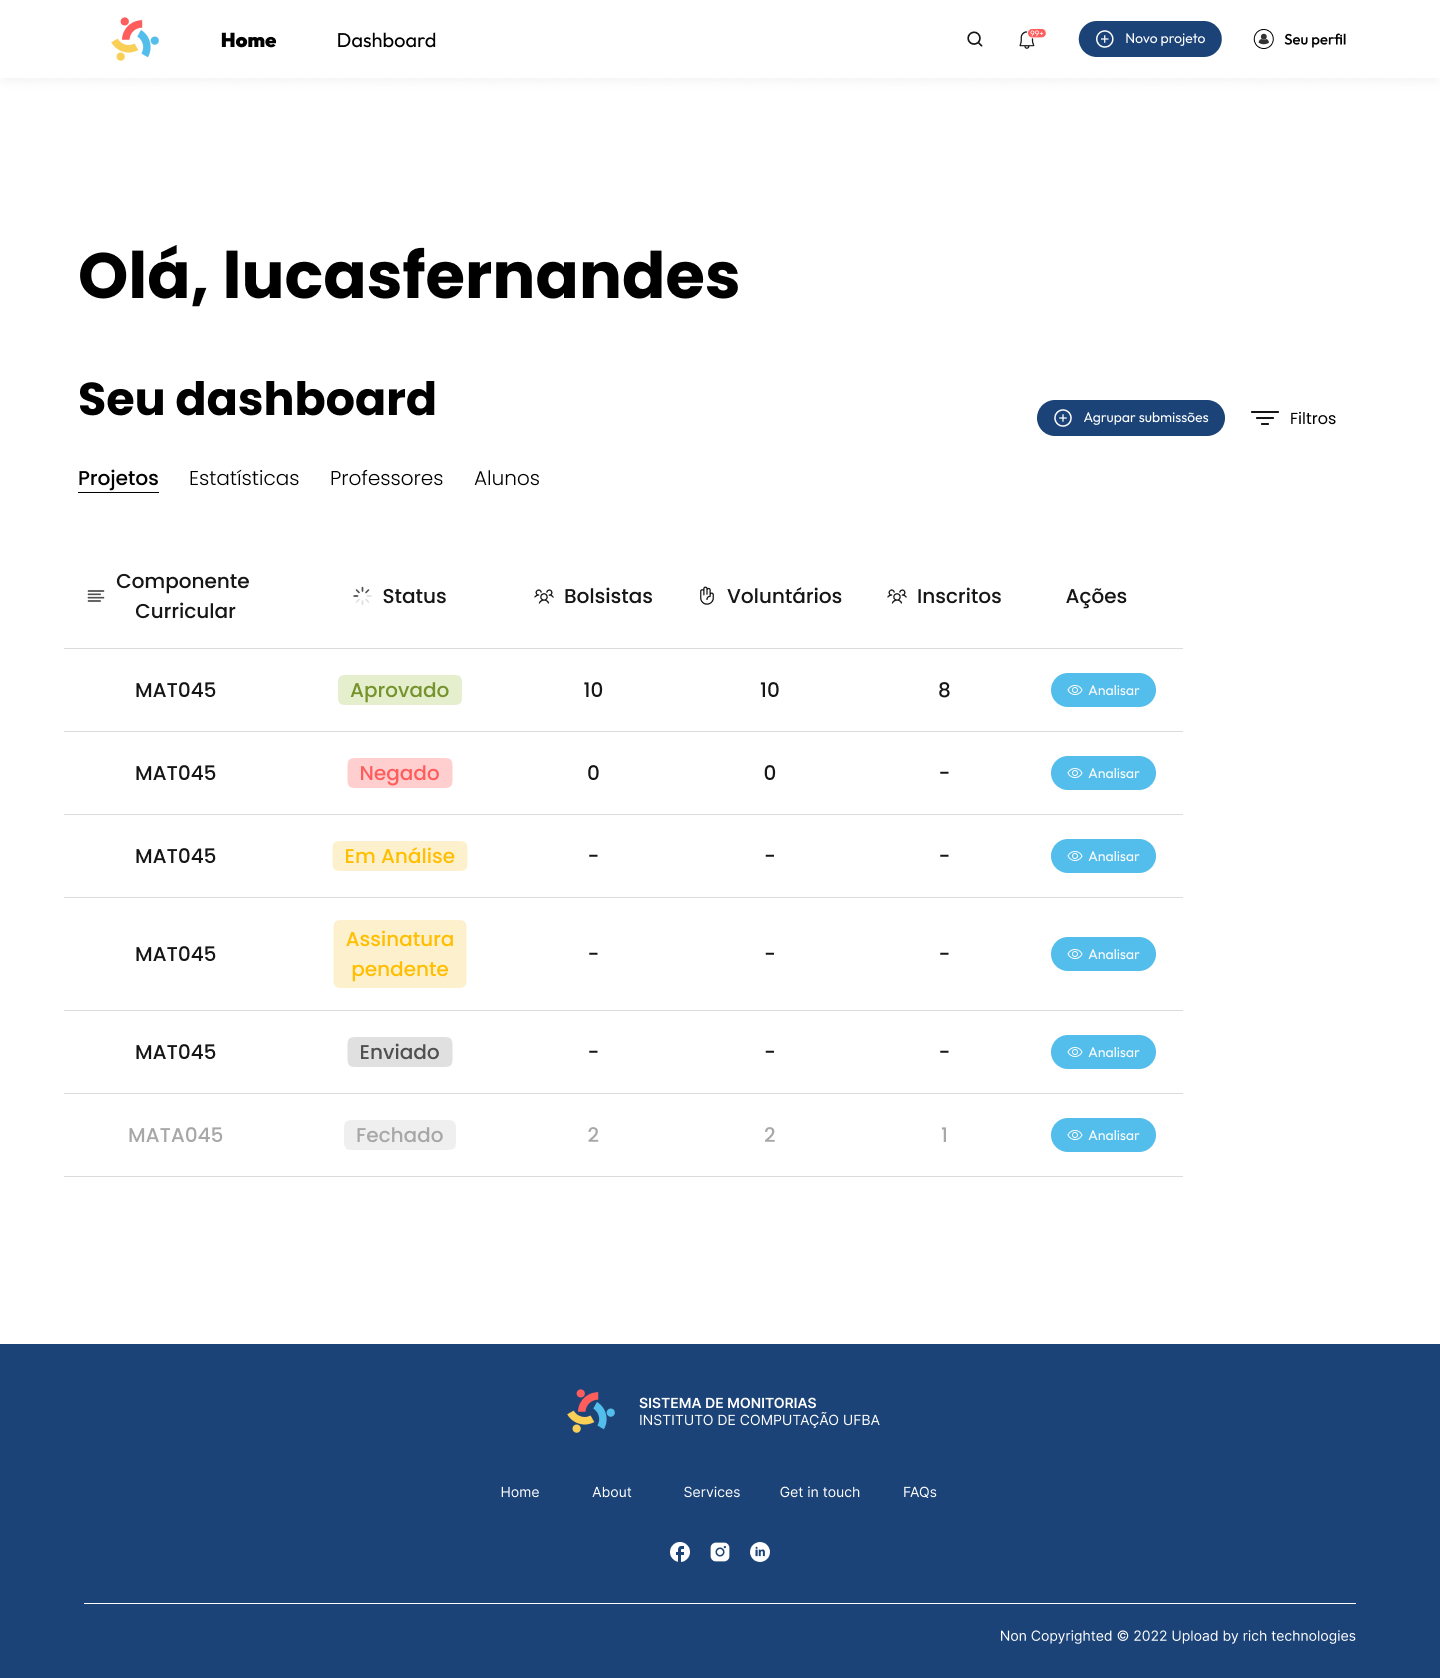
\includegraphics[width=0.8\textwidth]{figma/Dashboard_coodenador.png}
\caption{Dashboard do Coordenador - Visão de Projetos}
\label{fig:dashboard}
\end{figure}

\textbf{Decisões de Design}:
\begin{itemize}
    \item \textbf{Visão Consolidada}: Lista de todos os projetos com status visual claro
    \item \textbf{Filtros Rápidos}: Opções para filtrar por status (pendente, aprovado, em análise)
    \item \textbf{Ações em Lote}: Possibilidade de aprovar múltiplos projetos
    \item \textbf{Informações Essenciais}: Exibição de dados críticos (professor, disciplina, data de submissão)
    \item \textbf{Acesso Rápido}: Links diretos para visualizar detalhes de cada projeto
\end{itemize}

\subsection{Paleta de Cores}

\begin{figure}[H]
\centering
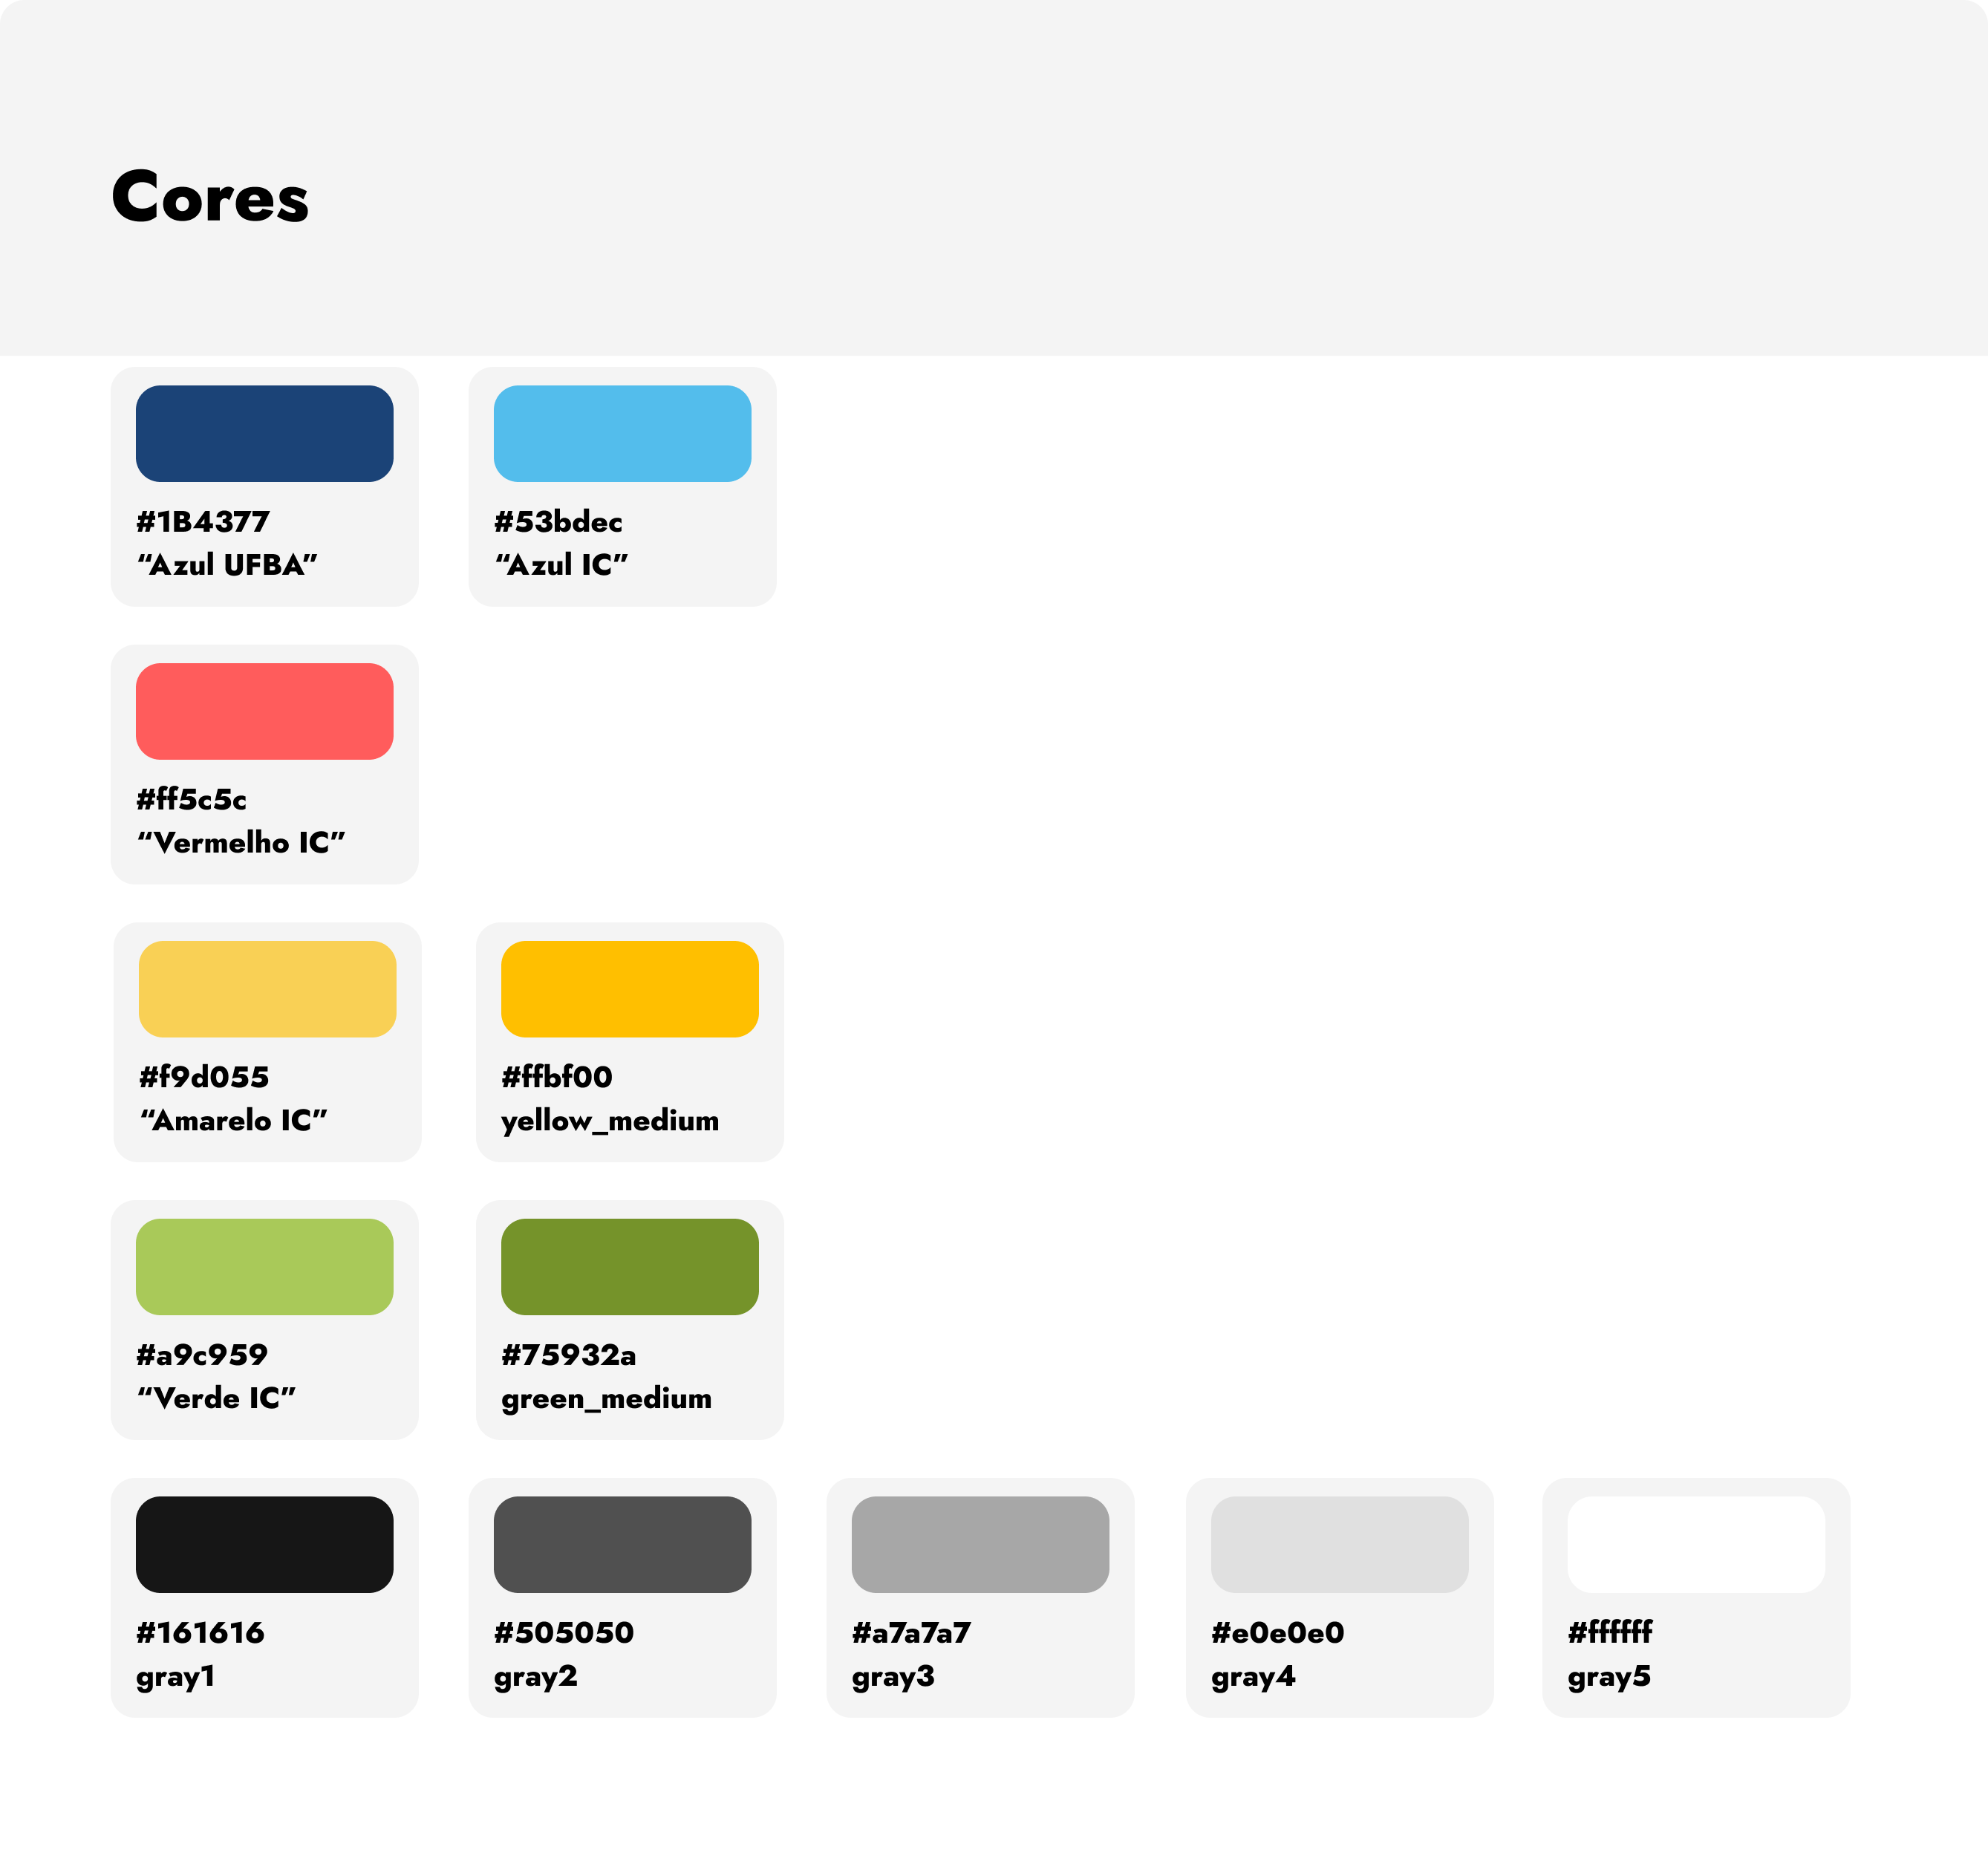
\includegraphics[width=0.8\textwidth]{figma/Cores.png}
\caption{Paleta de Cores Utilizada no Sistema}
\label{fig:cores}
\end{figure}

\textbf{Justificativa da Paleta}:
\begin{itemize}
    \item \textbf{Azul Institucional}: Cor primária da UFBA mantida para consistência
    \item \textbf{Verde de Aprovação}: Para indicar projetos aprovados e ações positivas
    \item \textbf{Amarelo de Pendência}: Para projetos aguardando análise
    \item \textbf{Cinzas Neutros}: Para elementos de interface e textos secundários
    \item \textbf{Alto Contraste}: Garantia de acessibilidade visual
\end{itemize}

\subsection{Tipografia}

\begin{figure}[H]
\centering
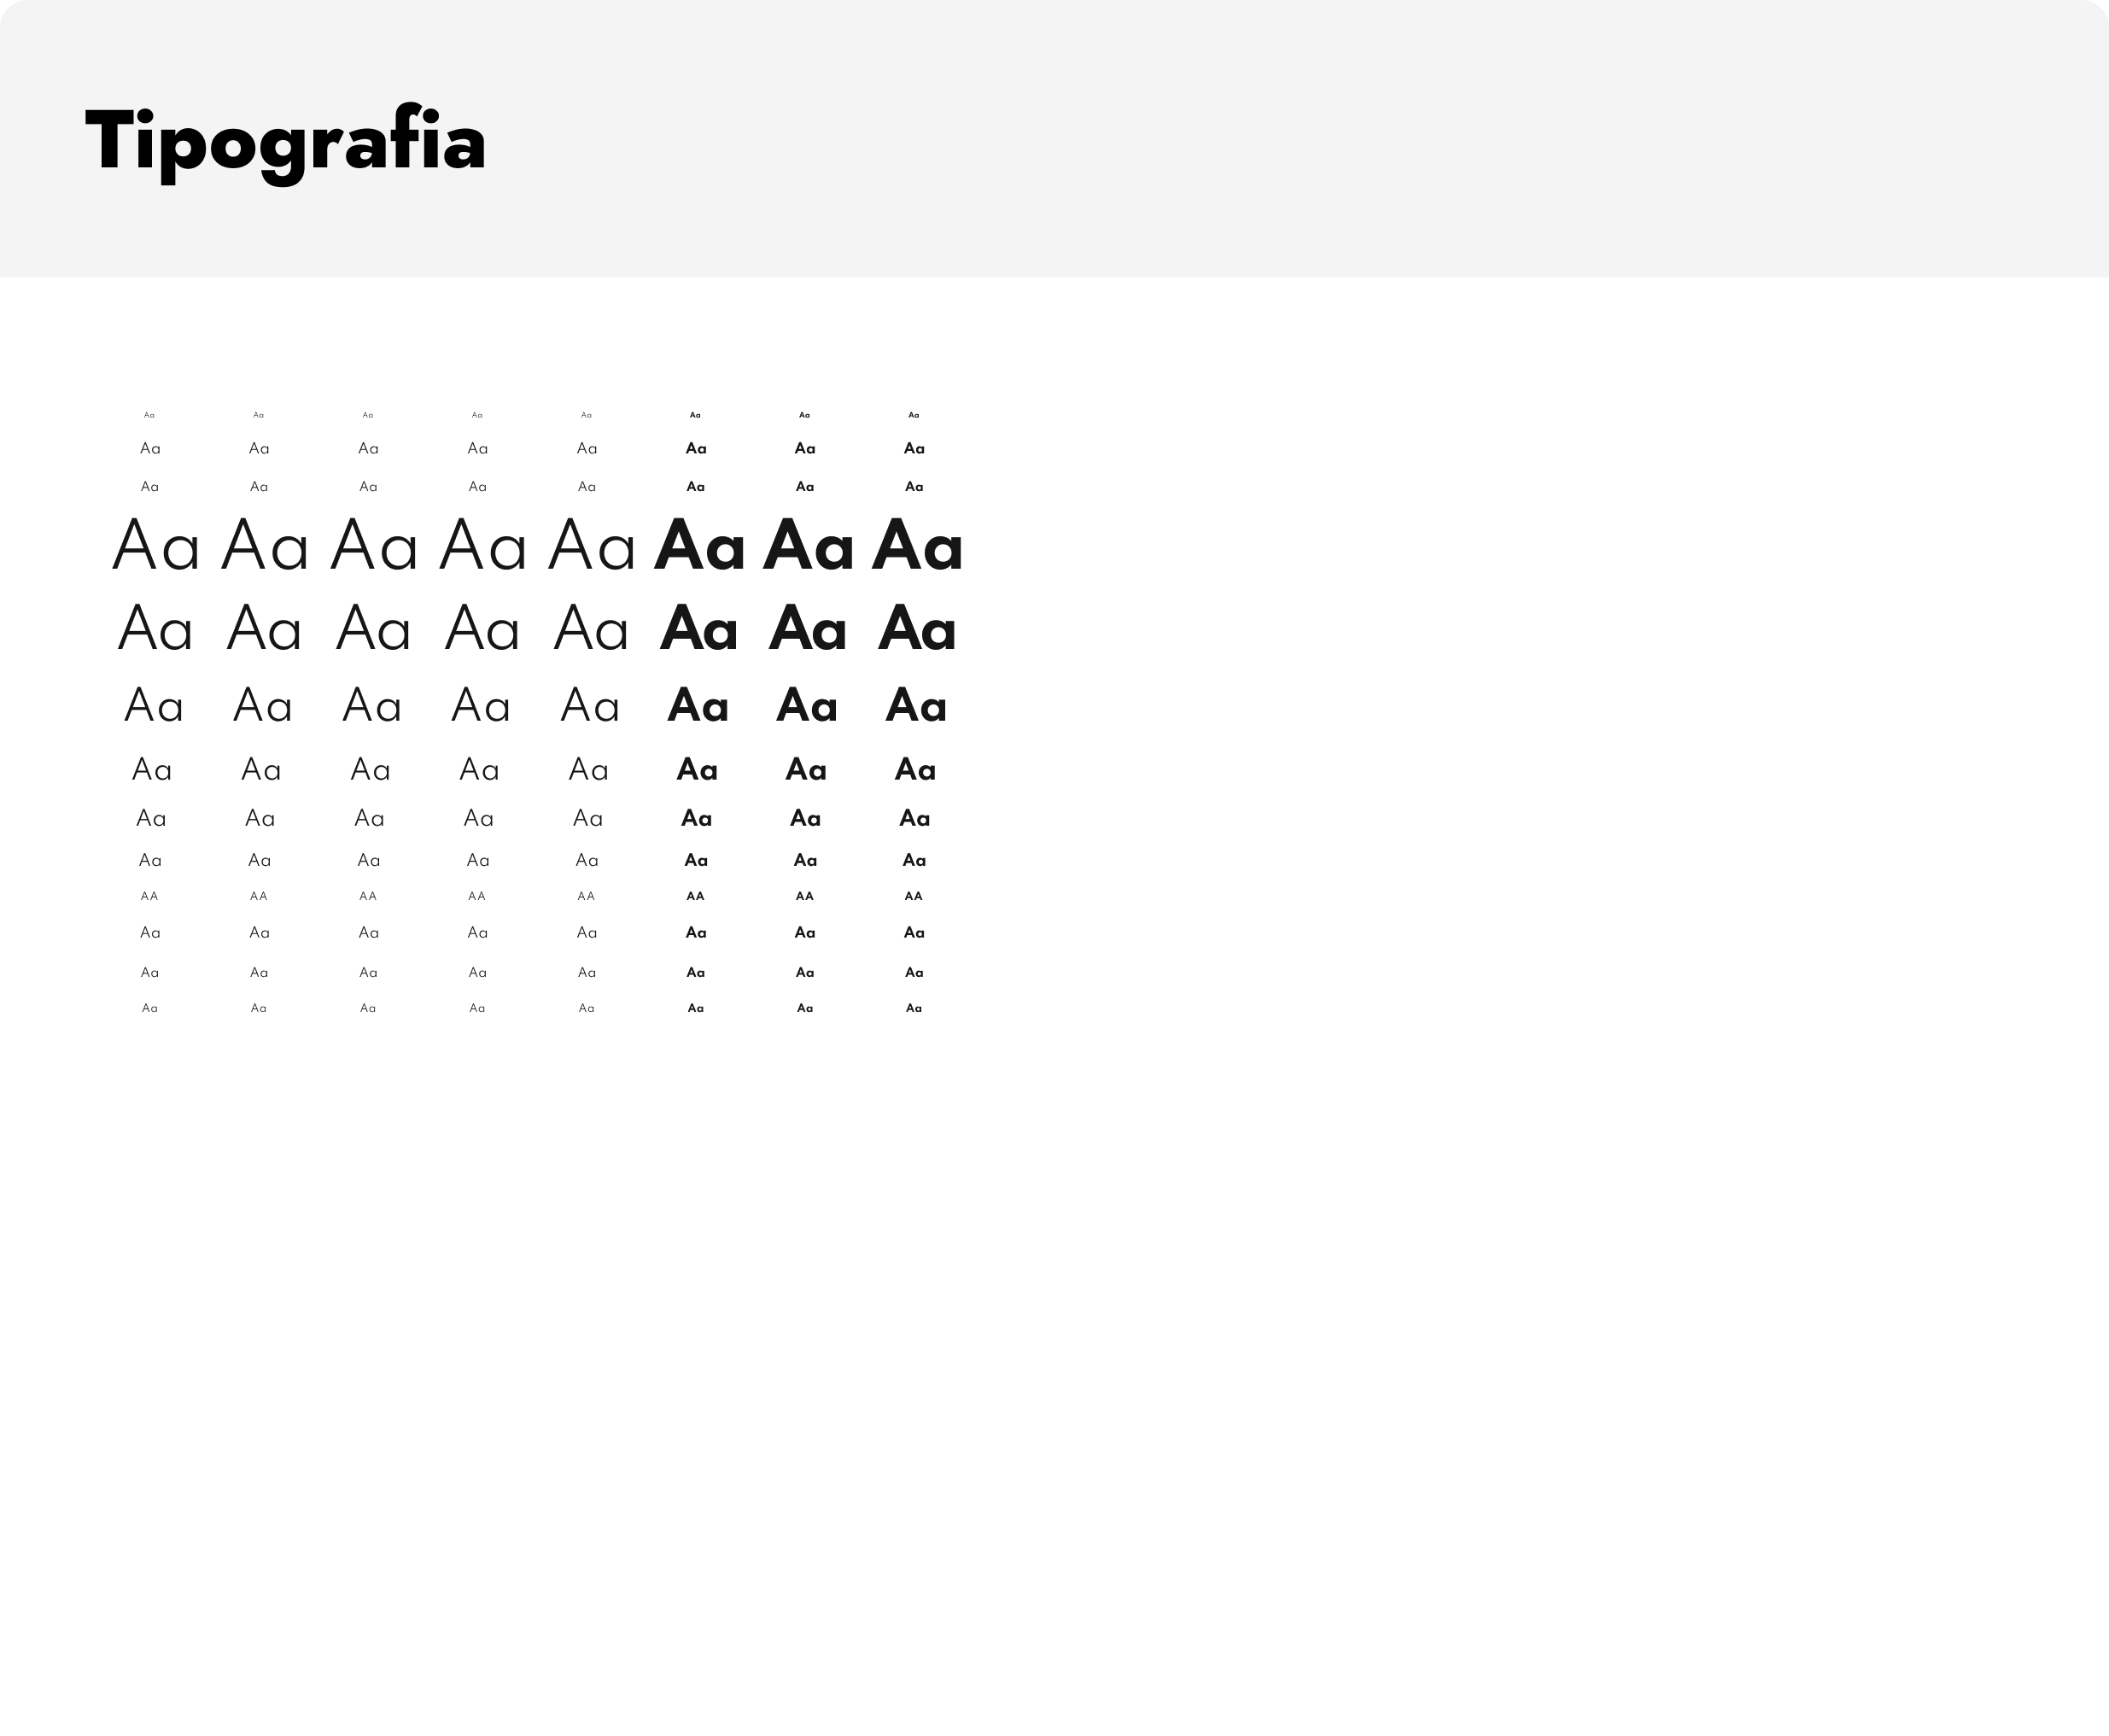
\includegraphics[width=0.8\textwidth]{figma/Tipografia.png}
\caption{Sistema Tipográfico do SIGA-M}
\label{fig:tipografia}
\end{figure}

\textbf{Decisões Tipográficas}:
\begin{itemize}
    \item \textbf{Hierarquia Clara}: Títulos, subtítulos e corpo de texto bem diferenciados
    \item \textbf{Legibilidade}: Fontes sans-serif para leitura em tela
    \item \textbf{Consistência}: Mesmo sistema tipográfico em todo o protótipo
    \item \textbf{Tamanhos Adequados}: Mínimo de 14px para corpo de texto
\end{itemize}

\section{Princípios de Design Aplicados}

\subsection{Foco na Tarefa Principal}

O protótipo foi desenvolvido com foco absoluto no fluxo crítico:

\begin{itemize}
    \item \textbf{Eliminação de Complexidade}: Apenas funcionalidades essenciais implementadas
    \item \textbf{Caminho Direto}: Mínimo de cliques para completar tarefas principais
    \item \textbf{Clareza de Propósito}: Cada tela tem objetivo único e claro
    \item \textbf{Feedback Imediato}: Confirmações visuais para cada ação importante
\end{itemize}

\subsection{Usabilidade Simplificada}

Considerações especiais para o contexto acadêmico:

\begin{itemize}
    \item \textbf{Familiaridade}: Interface similar a outros sistemas da UFBA
    \item \textbf{Linguagem Clara}: Terminologia alinhada com documentos oficiais
    \item \textbf{Processo Guiado}: Fluxo linear sem ramificações desnecessárias
    \item \textbf{Recuperação Fácil}: Sempre possível corrigir erros sem perder trabalho
\end{itemize}

\chapter{Etapa 3: Avaliação (Situação nova)}
\label{ch:avaliacao}

Esta etapa apresenta a avaliação do protótipo do sistema SIGA-M com potenciais usuários, verificando se os critérios de qualidade de IHC foram atendidos e se os requisitos definidos na análise foram contemplados.

\section{Método de Avaliação e Critérios}

\subsection{Método Escolhido: Teste de Usabilidade}

\textbf{TODO: [ESPECIFICAR DETALHES DO MÉTODO DE TESTE DE USABILIDADE APLICADO]}

O método de Teste de Usabilidade foi escolhido para avaliar o protótipo, pois permite observar diretamente como os usuários interagem com o sistema e identificar problemas práticos de usabilidade.

\subsection{Participantes}

\textbf{TODO: [DETALHAR PERFIL DOS PARTICIPANTES REAIS DA AVALIAÇÃO]}

A avaliação será conduzida com participantes representando os perfis de usuários identificados:
\begin{itemize}
    \item Professores do Instituto de Computação
    \item Membros de comissão de monitoria
\end{itemize}

\subsection{Critérios de Qualidade de Uso}

Os seguintes critérios de qualidade serão avaliados:

\subsubsection{Eficácia}
\begin{itemize}
    \item Taxa de sucesso na conclusão das tarefas principais
    \item Capacidade de alcançar os objetivos propostos
\end{itemize}

\subsubsection{Eficiência}
\begin{itemize}
    \item Tempo médio para completar cada tarefa
    \item Número de cliques/ações necessárias
    \item Fluidez na navegação
\end{itemize}

\subsubsection{Satisfação}
\begin{itemize}
    \item Avaliação subjetiva da experiência (escala Likert 1-5)
    \item Facilidade percebida de uso
    \item Confiança no sistema
\end{itemize}

\subsection{Instrumento de Coleta de Dados}

\textbf{TODO: [INSERIR QUESTIONÁRIO/ROTEIRO DE AVALIAÇÃO UTILIZADO]}

O instrumento de coleta incluirá:
\begin{itemize}
    \item Roteiro de tarefas a serem executadas
    \item Questionário pós-teste com escalas de satisfação
    \item Espaço para comentários qualitativos
\end{itemize}

\section{Análise da Avaliação Recebida}

\subsection{Resultados Quantitativos}

\textbf{TODO: [INSERIR DADOS REAIS DA AVALIAÇÃO]}
\begin{itemize}
    \item Taxas de sucesso por tarefa
    \item Tempos médios de execução
    \item Pontuações de satisfação
    \item Estatísticas de usabilidade
\end{itemize}

\subsection{Resultados Qualitativos}

\textbf{TODO: [INSERIR FEEDBACK QUALITATIVO DOS USUÁRIOS]}
\begin{itemize}
    \item Problemas de usabilidade identificados
    \item Comentários dos usuários
    \item Sugestões de melhoria
    \item Padrões de comportamento observados
\end{itemize}

\subsection{Mudanças Implementadas}

\textbf{TODO: [DETALHAR MUDANÇAS FEITAS NO PROTÓTIPO BASEADAS NO FEEDBACK]}

Com base no feedback recebido, as seguintes mudanças foram/serão implementadas:
\begin{itemize}
    \item Ajustes na interface
    \item Melhorias no fluxo de navegação
    \item Correções de problemas identificados
\end{itemize}

\subsection{Mudanças Não Implementadas}

\textbf{TODO: [JUSTIFICAR MUDANÇAS SUGERIDAS QUE NÃO FORAM IMPLEMENTADAS]}

Algumas sugestões não puderam ser implementadas pelos seguintes motivos:
\begin{itemize}
    \item Limitações técnicas do protótipo
    \item Escopo do projeto
    \item Restrições de tempo
\end{itemize}

\chapter{Etapa 4: Relato da Experiência}
\label{ch:relato}

Esta etapa apresenta o relato da experiência de desenvolvimento do projeto, incluindo o processo de trabalho da equipe e as reflexões sobre o aprendizado em IHC.

\section{Diário de Bordo}

Este diário documenta o processo completo de desenvolvimento do projeto SIGA-M, desde a concepção inicial até a finalização, registrando as contribuições específicas de cada membro da equipe e os marcos importantes do trabalho colaborativo.

\subsection{Processo de Desenvolvimento}

O projeto foi desenvolvido ao longo de 4 semanas intensivas, com uma divisão clara de responsabilidades que permitiu aproveitar as competências específicas de cada membro da equipe.

\subsubsection{Divisão de Responsabilidades}

\textbf{TODO: [CONFIRMAR/AJUSTAR DIVISÃO REAL DE TAREFAS]}

A equipe se organizou da seguinte forma:

\begin{itemize}
    \item \textbf{Antoniel Magalhães}: [DETALHAR CONTRIBUIÇÕES]
    \item \textbf{André Costa}: [DETALHAR CONTRIBUIÇÕES]
    \item \textbf{João Leahy}: [DETALHAR CONTRIBUIÇÕES]
    \item \textbf{Luis Felipe}: Documentação técnica e estruturação do relatório em LaTeX
    \item \textbf{Koichi Filho}: [DETALHAR CONTRIBUIÇÕES]
\end{itemize}

\subsection{Cronograma de Atividades Realizadas}

\begin{table}[H]
\centering
\begin{tabular}{|l|l|l|}
\hline
\textbf{Período} & \textbf{Atividade} & \textbf{Responsáveis} \\
\hline
9-15 Jun & Definição do tema e análise de requisitos & Todos \\
\hline
16-18 Jun & Criação de personas e cenários & [TODO] \\
\hline
19-25 Jun & Desenvolvimento da HTA & [TODO] \\
\hline
26 Jun-7 Jul & Design do protótipo no Figma & [TODO] \\
\hline
1-8 Jul & Preparação da avaliação & [TODO] \\
\hline
9 Jul & Aplicação da avaliação & Todos \\
\hline
10-13 Jul & Análise dos resultados e finalização & Todos \\
\hline
\end{tabular}
\caption{Cronograma de Atividades da Equipe}
\label{tab:cronograma}
\end{table}

\subsection{Lições Aprendidas}

\subsubsection{Sobre Colaboração em Design}

\textbf{TODO: [ADICIONAR REFLEXÕES REAIS DA EQUIPE]}

\begin{itemize}
    \item Importância da comunicação clara
    \item Valor da divisão de tarefas por competências
    \item Necessidade de revisões constantes
\end{itemize}

\subsubsection{Sobre Design de IHC}

\textbf{TODO: [ADICIONAR APRENDIZADOS ESPECÍFICOS DE IHC]}

\begin{itemize}
    \item Importância do design centrado no usuário
    \item Valor dos protótipos iterativos
    \item Necessidade de validação com usuários reais
\end{itemize}

\section{Autoavaliação}

\subsection{Avaliação da Equipe}

\textbf{TODO: [DISCUTIR E DEFINIR NOTA COLETIVA]}

A equipe demonstrou:
\begin{itemize}
    \item Colaboração efetiva
    \item Cumprimento de prazos
    \item Qualidade nas entregas
    \item Aprendizado conjunto
\end{itemize}

\textbf{Nota da Equipe}: [DEFINIR]/10

\subsection{Avaliação Individual}

\textbf{TODO: [CADA MEMBRO DEVE FORNECER SUA AUTOAVALIAÇÃO]}

\subsubsection{Antoniel Magalhães}
\textbf{Contribuições}: [DETALHAR]
\textbf{Nota Individual}: [DEFINIR]/10

\subsubsection{André Costa}
\textbf{Contribuições}: [DETALHAR]
\textbf{Nota Individual}: [DEFINIR]/10

\subsubsection{João Leahy}
\textbf{Contribuições}: [DETALHAR]
\textbf{Nota Individual}: [DEFINIR]/10

\subsubsection{Luis Felipe}
\textbf{Contribuições}: Documentação técnica, estruturação LaTeX, organização das entregas
\textbf{Nota Individual}: [DEFINIR]/10

\subsubsection{Koichi Filho}
\textbf{Contribuições}: [DETALHAR]
\textbf{Nota Individual}: [DEFINIR]/10

\end{document} 